\documentclass[11pt]{article}

\usepackage[francais]{babel}
\usepackage[margin=25mm]{geometry}
\usepackage{amsmath}
\usepackage{hyperref}
\usepackage{mathtools, bm}
\usepackage{amssymb, bm}
\usepackage{amsthm}
\usepackage{algorithm}
\usepackage{algorithmic}
\usepackage[utf8]{inputenc}
\usepackage{calrsfs}
\usepackage{xcolor}
\usepackage[T1]{fontenc}
\usepackage{caption}
\usepackage{listings}
\usepackage{graphicx} 
\usepackage{fancyvrb} 
\usepackage{listings} 
\usepackage{bm} 
\usepackage{xcolor}


\newtheorem{theorem}{Théorème}
\newtheorem{corollary}[theorem]{Corollaire}
\newtheorem{lemma}[theorem]{Lemme}
\newtheorem{definition}[theorem]{Définition}
\newtheorem{example}[theorem]{Exemple}
\newtheorem{property}[theorem]{Propriété}
\newtheorem{remark}[theorem]{Remarque}
\captionsetup[algorithm]{name=Algorithme}

\let\vega\vartheta

 
\definecolor{dkgreen}{rgb}{0,0.6,0} %for listings
\definecolor{gray}{rgb}{0.5,0.5,0.5} %for listings
\definecolor{mauve}{rgb}{0.58,0,0.82} %for listings

% Des styles pour afficher le code R, piqué sur le web OFC

\lstset{ % 
  language=R,                % the language of the code 
  basicstyle=\footnotesize,           % the size of the fonts that are used for the code 
%  numbers=left,                   % where to put the line-numbers 
%  numberstyle=\tiny\color{gray},  % the style that is used for the line-numbers 
%  stepnumber=2,                   % the step between two line-numbers. If it's 1, each line 
                                  % will be numbered 
%  numbersep=5pt,                  % how far the line-numbers are from the code 
  backgroundcolor=\color{white},      % choose the background color. You must add \usepackage{color} 
  showspaces=false,               % show spaces adding particular underscores 
  showstringspaces=false,         % underline spaces within strings 
  showtabs=false,                 % show tabs within strings adding particular underscores 
  frame=single,                   % adds a frame around the code 
  rulecolor=\color{black},        % if not set, the frame-color may be changed on line-breaks within not-black text (e.g. commens (green here)) 
  tabsize=2,                      % sets default tabsize to 2 spaces 
  captionpos=b,                   % sets the caption-position to bottom 
  breaklines=true,                % sets automatic line breaking 
  breakatwhitespace=false,        % sets if automatic breaks should only happen at whitespace 
  title=\lstname,                   % show the filename of files included with \lstinputlisting; 
                                  % also try caption instead of title 
  keywordstyle=\color{blue},          % keyword style 
  commentstyle=\color{dkgreen},       % comment style 
  stringstyle=\color{mauve},         % string literal style 
  escapeinside={\%*}{*)},            % if you want to add a comment within your code 
  morekeywords={*,...}               % if you want to add more keywords to the set 
} 



\begin{document}
%*******************************************************
% Titlepage
%*******************************************************
\begin{titlepage}
	\centering

	{\scshape\LARGE Institut de Science Financière et d'Assurances	 \par}\vspace{1cm}
   	 
\includegraphics[width=0.55\textwidth]{logo_isfa}\par
	\vspace{1.5cm}
	{\scshape\Large Projet\par}
	\vspace{1.5cm}
	{\huge\bfseries Théorie financière\par}
	\vspace{2cm}{W. LAURENT, O. LAVERNY, P. MARJOLLET\par}
	\vfill
	\par
	\textsc{Pr. JIAO YING}

	\vfill

% Bottom of the page
	{\large \today\par}
\end{titlepage}

\begin{abstract}
Après avoir rappelé la dynamique du taux court, sa solution dans le modèle Vasicek, ainsi quelques considérations à propos des processus d'Ornstein-Uhlenbeck, nous nous interessons au modèle à un facteur : le modèle de Hull et White. Nous en rappelons la dynamique de taux court, calculons la forme explicite de du taux court en en résolvant l'équation différentielle stochastique, calculons ensuite le prix du zero coupon ainsi que les taux d'interet continu moyen.Finalement, nous traçons la surface de taux correspondante en prenant des paramètres arbitraires. 
\end{abstract}

\tableofcontents

\section{Introduction}
Nous allons traiter ici le modèle d'Hull et White, développé à partir du modèle de Vasicek en 1990. Nous commencerons par quelques prérequis, notamment le modèle de vasicek ainsi que des considérations sur les processus d'Ornstein-Uhlenbeck correspondant, avant de nous attaquer au modèle HW en lui-même. Rappelons que nous nous plaçons dans un modèle de marché parfait (infinie liquidité des actifs, coûts de transaction nuls, actifs infiniment divisibles notamment).

\section{Le modèle de vasicek et quelques pré-requis}
%Developped by John C. Hull and Alan White in 1990, the hull-white model is still popular in the market today. At first, they wanted a model that fits the term structure better than the Vasicek model. The need of fit lead us to add a time-depending deterministic parameter  In it's most extensive and general form, it's 


Rappelons ici la dynamique du taux court dans le modèle de vasicek: 

\begin{definition}[Dynamique du taux court sous Vasicek]
Sous le modèle de vasicek, le taux court suit la dynamique suivante: 
\begin{center}
$dr_{t} = a(b-r_{t})dt + \sigma dW_{t}$
\end{center}
Avec :
\begin{itemize}
  \item $a$ constante positive, représentant la force de rappel
  \item $b$ constante positive, représentant le taux long terme
  \item $\sigma$ constante positive, représentant la volatilité
\end{itemize}
On pourrait tout a fait noter $\vega = ab$, les paramètres du modèle devenant alors $\vega$, $a$ et $\sigma$
\end{definition}

Sous vasicek, le taux court suit un processus d'Ornstein-Uhlenbeck, et la solution correspondante est : 
\begin{theorem}[Solution de la dynamique du taux court Vasicek]
\begin{displaymath}
r_t = r_0 e^{-at} + b(1-e^{-at}) + \sigma e^{-at} \int_0^t e^{au} dW_u
\end{displaymath}
\end{theorem}

\begin{remark} \label{O-U}
A t fixé, ce processus d'Ornstein-Uhlenbeck suit une loi gaussienne de paramètres son espérance et sa variances, un processus d'Ornstein-Uhlenbeck est en effet à la fois Gaussien et Markovien. 
\end{remark}

\begin{property}[Espérance de l'exponentielle d'une loi normale]
Soit $X$ une variable aléatoire suivant une loi normale. Alors $e^X$ suit une loi log-normale et donc :
\begin{center}
$\mathbb{E}(e^X) = e^{\mathbb{E}(X) + \frac{1}{2} \mathbb{V}(X)}$
\end{center}
\end{property}









\section{Le modèle de Hull et White}
Développé par J.C.Hull et A.White a partir de 1990, le modèle Hull-White est encore très utilisé sur le marché aujourd'hui. L'objectif premier de ce modèle était de correspondre exactement aux données de marché afin de d'obtenir une courbe des taux dans le modèle correspondant exactement à la courbe empirique des taux "réels" fournie par le marché. L'intuition fut la suivante : ajouter un paramètre (non-stochastique) dépendant du temps dans le \emph{drift} de la dynamique du taux d'intérêt. La mise en oeuvre de ce modèle nécessite une paramétrisation (le paramètre non-stochastique ajouté) à partir des données de marché. 



Dans l'extension proposée par Hull-white du modèle de vasicek, c'est le paramètre $\vega$ qui devient une fonction déterministe du temps : 

\begin{definition}[Dynamique du taux court sous Hull-White]
Sous le modèle Hull-White, le taux court suit la dynamique suivante : 
\begin{center}
$dr_{t} = (\vega_{t}-ar_{t})dt + \sigma dW_{t}$
\end{center}
Avec :
\begin{itemize}
  \item $a$ constante positive, représentant la force de rappel
  \item $\vega_{t}$ une fonction déterministe du temps
  \item $\sigma$ constante positive, représentant la volatilité
\end{itemize}
\end{definition}

\begin{property}
	Par intégration (via le lemme d'Ito) de la dynamique du taux court sous Hull-White, on obtient: \ 
    \begin{displaymath}
    	r_t = r_{s}e^{-a(t-s)}+\int_s^t e^{-a(t-u)}\vega_u du + \sigma \int_s^t e^{-a(t-u)}dW_u
    \end{displaymath}
    \begin{proof}
    	On a: 
        \begin{align*}
			d(r_{t}e^{at})  &= r_{t}e^{at}adt + e^{at}dr_{t} \\
           					&= r_{t}e^{at}adt + e^{at}\vega_{t}dt - r_{t}e^{at}adt + e^{at}\sigma dW_{t} \\
           					&= e^{at}(\vega_{t}dt+\sigma dW_{t})
		\end{align*}
		
        Ce qui implique que : 
\begin{center}
        $r_{t}e^{at}  = r_{s}e^{as}+\int_s^t e^{au}\vega_u du + \sigma \int_s^t e^{au}dW_u$
        \end{center}
        et donc : 
        \begin{center}
			$r_t = r_{s}e^{-a(t-s)}+\int_s^t e^{-a(t-u)}\vega_u du + \sigma \int_s^t e^{-a(t-u)}dW_u$
        \end{center}
    \end{proof}
\end{property}



\begin{property} Sous le modèle Hull-White, le prix d'un zéro-coupon est donné par :
\begin{displaymath}
	B(t,T)=exp(\frac{ r_t (1-e^{-a(T-t)})}{a} - \frac{1}{a}\int_t^T \vega_u (1-e^{-a(T-u)}) du + \frac{1}{2}[\int_t^T \frac{{\sigma}^2}{a^2}(1-e^{-a(t-u)^2} du)])
\end{displaymath}

 
    \begin{proof}
    	On commence par calculer $\int_t^T r_s ds$ directement à partir de la dynamique de r :
        \begin{align*}
        	r_T - r_t & = \int_t^T \vega_u - a r_u du + \int_t^T\sigma d W_u \\
            		& = \int_t^T \vega_u du - \int_t^T ar_u du + \sigma\int_t^T dW_u
        \end{align*}
       	Remarquons que grâce a la propriété précédente, 
        
        \begin{align*}
        r_T - r_t & = r_{t}e^{-a(T-t)}+\int_t^T e^{-a(T-u)}\vega_u du + \sigma \int_t^T e^{-a(T-u)}dW_u - r_t \\
        & = -r_{t}(1-e^{-a(T-t)})+\int_t^T e^{-a(T-u)}\vega_u du + \sigma \int_t^T e^{-a(T-u)}dW_u \\
        \end{align*}
        
        Que l'on injectera dans notre équation : 
        \begin{align*}
        	a \int_t^T r_u du & = \int_t^T \vega_u du - ( r_T - r_t ) + \sigma\int_t^T dW_u \\
              				 & = \int_t^T \vega_u du - ( - r_{t}(1-e^{-a(T-t)})+\int_t^T e^{-a(T-u)}\vega_u du + \sigma \int_t^T e^{-a(T-u)}dW_u )+ \sigma\int_t^T dW_u \\
							 & =  r_{t}(1-e^{-a(T-t)}) + \int_t^T \vega_u (1-e^{-a(T-u)}) du + \sigma \int_t^T (1-e^{-a(T-u)}) dW_u 
		\end{align*}
        Finalement, on a:
        \begin{displaymath}
        	\int_t^T r_u du = \frac{ r_t (1-e^{-a(T-t)})}{a} + \frac{1}{a}\int_t^T \vega_u (1-e^{-a(T-u)}) du + \frac{\sigma}{a} \int_t^T (1-e^{-a(T-u)}) dW_u 
        \end{displaymath}
        Calculons son espérance, en notant que l'intégrale sur le brownien est une martingale (d'espérance nulle) :
        \begin{align*}
        	\mathbb{E}[\int_t^T r_u du | \mathcal{F}_t] & = \frac{ r_t (1-e^{-a(T-t)})}{a} + \frac{1}{a}\int_t^T \vega_u (1-e^{-a(T-u)}) du + \underbrace{\mathbb{E}[\frac{\sigma}{a} \int_t^T (1-e^{-a(T-u)}) dW_u|\mathcal{F}_t]}_{=0}\\
            & = \frac{ r_t (1-e^{-a(T-t)})}{a} + \frac{1}{a}\int_t^T \vega_u (1-e^{-a(T-u)}) du
        \end{align*}
    	Ainsi que sa variance :
        \begin{center}
        $Var[\int_t^T r_u du | \mathcal{F}_t] = Var[ \underbrace{\frac{ r_t (1-e^{-a(T-t)})}{a}}_{deterministe} + \underbrace{\frac{1}{a}\int_t^T \vega_u (1-e^{-a(T-u)}) du}_{deterministe} + \underbrace{\frac{\sigma}{a} \int_t^T (1-e^{-a(T-u)}) dW_u}_{stochastique}]$
        \end{center}
        Et ainsi : 
        \begin{align*}
        Var[\int_t^T r_u du | \mathcal{F}_t] & = Var[\frac{\sigma}{a} \int_t^T (1-e^{-a(T-u)}) dW_u] \\
           									 & = \int_t^T \frac{{\sigma}^2}{a^2}(1-e^{-a(t-u)})^2 du
        \end{align*}
        
        
        Comme $\int_t^T r_u du | \mathcal{F}_t$ est un processus d'Ornstein-Uhlenbeck, on utilise la propriété \ref{O-U}, et on obtient :
        \begin{align*}
        	B(t,T)  & = \mathbb{E}[e^{-\int_t^T r_s ds}|\mathcal{F}_s] \\
            	& = exp(-\mathbb{E}[\int_t^T r_u du | \mathcal{F}_t] + \frac{1}{2}Var[\int_t^T r_u du | \mathcal{F}_t]) \\
                & = exp(\frac{ r_t (1-e^{-a(T-t)})}{a} - \frac{1}{a}\int_t^T \vega_u (1-e^{-a(T-u)}) du + \frac{1}{2}[\int_t^T \frac{{\sigma}^2}{a^2}(1-e^{-a(t-u)^2} du)])
        \end{align*}
    \end{proof}
    
    
\end{property}

Ainsi, nous avons pu complètement définir le prix de n'importe quel zéro-coupon. Pour des raisons de simplification des calculs, nous prendrons les notation suivante : 

\begin{center}
$\forall t,T, A(t,T) = \frac{1-e^{-a(T-t)}}{a}$

$\forall t,T, C(t,T) = - \int_t^T \vega_u A(u,T) + \frac{ \sigma^2 A(u,T)^2}{2} du$
\end{center}

Et le prix du zéro coupon s'écrit alors : 


\begin{center}
$B(t,T)  = \exp{ - r_t A(t,T) + C(t,T)}$
\end{center}

\begin{remark}
On voit ici que le modèle de Hull-White à un facteur est bien un modèle affine, étant donné que $\exp{C(t,T)}$ et $A(t,T)$ sont des fonctions déterministes.
\end{remark}

Pour en arriver a notre but (construire la courbe des taux), nous allons maintenant déduire du prix du zéro-coupon le prix des taux moyens continus : 

\begin{property} [Taux d'intérêt continu moyen]
Par définition, le taux d'intérêt continu moyen s'écrit : 
\begin{displaymath}
R(t,T) = \frac{-1}{T-t} ln(B(t,T))
\end{displaymath}

Ici, on a : 
\begin{displaymath}
R(t,T) = \frac{-1}{T-t} ( - r_t A(t,T) + C(t,T))
\end{displaymath}

\end{property}



% %ajouter les taux forward, et éventuellement le prix d'un call ou put européen

% \section{Le zero-coupon comme numéraire}
% Sous le numéraire que nous avons jusque là, le cash, le zero coupon s'écrit : 
% \begin{center}
% $B(t,T)  = exp( r_t A(t,T) - \int_t^T \vega_u A(u,T) du + \frac{1}{2} \int_t^T \sigma^2 A(u,T)^2 du)$
% \end{center}

% Nous pourrions utiliser le zero coupon de maturité $T$ fixée comme numéraire. 

% La densité de radon-nikodym corespondante a ce changement de probabilité est : 

% \begin{align*}
% \eta_t & = \frac{B(t,T)}{e^{\int_0^t r_s ds}} \frac{1}{B(0,T)} \\
% 	   & = exp\{ r_t A(t,T) - \int_t^T \vega_u A(u,T) du + \frac{1}{2} \int_t^T \sigma^2 A(u,T)^2 du - \int_0^t r_s ds - r_0 A(0,T) + \int_0^T \vega_u A(u,T) du - \frac{1}{2} \int_0^T \sigma^2 A(u,T)^2 du\} \\
% 	   & = exp\{ r_t A(t,T) + \int_0^t \vega_u A(u,T) du - \frac{1}{2} \int_0^t \sigma^2 A(u,T)^2 du - \int_0^t r_s ds - r_0 A(0,T) \} \\
%        & = exp\{ r_t A(t,T) + \int_0^t \vega_u A(u,T) du - \frac{1}{2} \int_0^t \sigma^2 A(u,T)^2 du - \int_0^t r_s ds - r_0 A(0,T) \}
% \end{align*}

% Qui est bien, par construction, une matringuale exponentielle d'experance 1. 

% \section{Formule de princing sous notre nouveau numeraire : le zero-coupon de maturité T }

% Sous ce nouveau numéraire, la formule de princing est la suivante : 

% \begin{definition}[Formule de pricing]
% Comme montrer en cours, un produit dérivé $X$ à pour prix sous notre nouveau numeraire :
% \begin{displaymath}
% X_t = B(t,T)\mathbb{E}_\mathbb{Q}(X_T \| \mathbb{F}_t)
% \end{displaymath}
% \end{definition}

% \begin{example}[Call sur le zero-coupon]
% Pour un call d'échéance $T$ et de strike $K$ sur notre zero-coupon, on a que : 
% \begin{align*}
% C_t & = B(t,T)\mathbb{E}_\mathbb{Q}[(B(T,U)-K)_+ | \mathcal{F}_t]
% 	& = exp( r_t A(t,T) - \int_t^T \vega_u A(u,T) du + \frac{1}{2} \int_t^T \sigma^2 A(u,T)^2 du) 
% \end{align*}

% Il faut ensuite calculer le prix de l'option par l'EDP correspondante... Je sais pas le faire ! 
% \end{example}


\section{Simulations}
Pour l'ensemble des simulations suivantes, nous avons arbitrairement fixé :\\
\begin{center}
$a=0.5$, $\sigma=1$, $r_0 = 0$ et $\vega(t) = 1-\frac{\sin(10t)}{t+1}$
\end{center}
Comme présenté précédemment, la mise en oeuvre de ce modèle nécessité une paramétrisation de $\vega$ à partir des données de marchés. Nous choisirons des fonctions simples pour $\vega$, sans pousser plus loin la paramétrisation du modèle avec les données de marché.
\begin{algorithm}[H]
\caption{Génération de notre processus de Wiener standard $W_{t}$}
On fixe le nombre de discrétisation de notre brownien $n$.\\
Soit $W$ notre vecteur contenant les valeurs du mouvement brownien\\
$W_{0}=0$ et pour $i$ de $1$ à $n-1$ : $W_{i+1} = W_{i} + \frac{1}{n} \cdot \eta$\\
Avec $\eta$ une réalisation d'une $\mathcal{N}(0,1)$ pour chaque itération de $i$.\\
\end{algorithm}

\begin{figure}[H]
         \centering 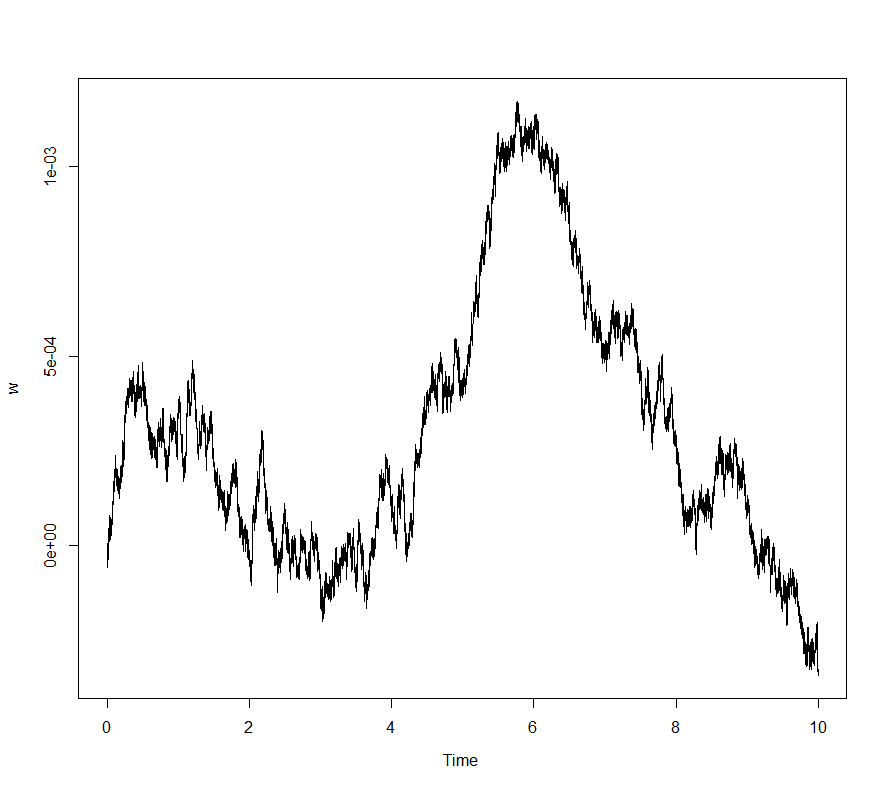
\includegraphics[scale=0.55]{graphbrown}
        \caption{Simulation d'un mouvement brownien sur 10 ans avec 1 000 000 itérations}
\end{figure}

\subsection{Simulation du taux court}
Maintenant que nous avons un brownien standard, nous pouvons nous en servir pour simuler le taux court $r_{t}$.
\begin{algorithm}[H]
\caption{Génération d'un taux court $r_{t}$}
On fixe $a$, $\sigma$ et $\vega$.\\
On génère un mouvement brownien $W$.\\
$tmp_1$ reçoit le calcul numérique de $\int^{t}_{0}e^{-a\cdot(t-u)}\cdot \vega(u) du$.\\
On décompose : $\int^{t}_{0}e^{au}dW_{u} = e^{at}W_{t} - \int^{t}_{0}a \cdot e^{au} \cdot W_u du$.\\
$tmp_2$ reçoit le calcul numérique de $\int^{t}_{0}a \cdot e^{au} \cdot W_{u} du$ (méthode des rectangles par exemple).\\
$r_{t}$ reçoit finalement $r_{0} \cdot e^{-at} + tmp_{1} + \sigma e^{-at} \cdot (e^{at} \cdot W_{t} - tmp_{2})$.
\end{algorithm}


Le graphique suivant représente le taux court en fonction du temps $t$ ainsi que de nos paramètres fixés préalablement. Notons que notre fonction $\vega$ nous permet d'obtenir un taux court qui croît globalement et qui oscille légèrement pour enfin visiblement converger (car $\vega$ est bornée).
\begin{figure}[H]
         \centering 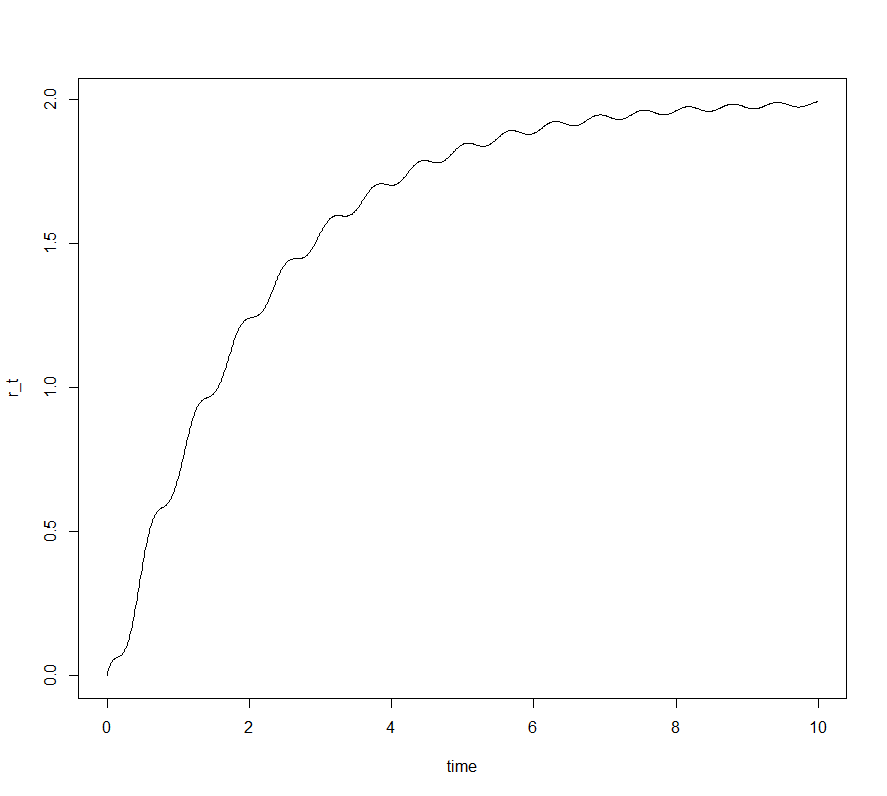
\includegraphics[scale=0.55]{taux_court}
        \caption{Simulation d'un taux court sur 10 ans avec 1 000 000 de discrétisations du brownien sousjacent}
\end{figure}

\noindent L'intérêt de la fonction sinus dans $\vega$ était d'avoir un caractère oscillatoire dans notre taux court, l'idée étant de se rapprocher de la réalité sans aller plus loin dans la paramétrisation.

\subsection{Simulation du prix du zéro-coupon $B(0,T)$}
\begin{algorithm}[H]
\caption{Calcul du prix d'un $ZC$ : $B(0,T)$}
Si $T=0$ alors $B(0,T)=1$.\\
On déclare $A(t,T,a) = \frac{1}{a} \cdot (1 - e^{-a\cdot (T-t)})$
Comme $r_{0} = 0$,  cela nous épargne le calcul de $tmp_{1} = r_{0} \cdot A(0,T,a)$.\\
$tmp_{2}$ reçoit le calcul numérique de $\int^{T}_{0} \vega(s) \cdot A(s,T,a) ds$\\
$tmp_{3}$ reçoit le calcul numérique de $\frac{1}{2} \cdot \sigma^{2} \cdot \int^{T}_{0}A(s,T,a)^2ds$\\
Enfin on a $B(0,T)=e^{tmp_{1} - tmp_{2} + tmp_{3}}$
\end{algorithm}


Le graphique suivant représente donc le prix d'un zéro-coupon $B(0,t)$ en $0$ en fonction de sa maturité $T$. Notons qu'ici le taux court n'est pas exploité. 
\begin{figure}[H]
         \centering 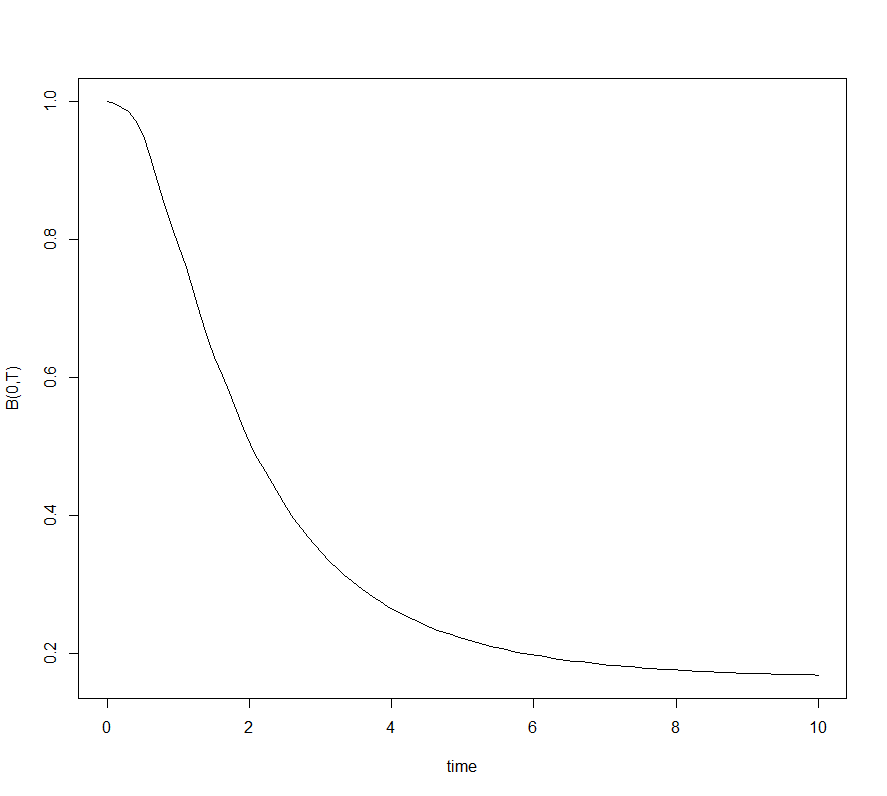
\includegraphics[scale=0.55]{0_C_en_0_de_mat_T}
        \caption{Simulation du prix d'un zéro-coupon de maturité $T$}
\end{figure}
Il est cohérent d'obtenir une fonction décroissante en T en t=0 fixé pour des taux d'intérêt positifs.


Et le suivant représente le prix d'un zéro-coupon $B(t,T)$
\begin{center}
\begin{figure}[H]
        \centering 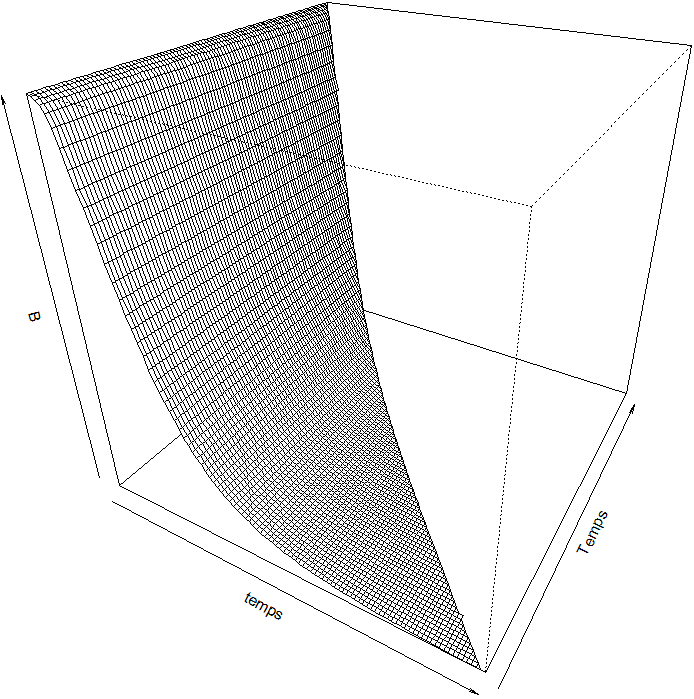
\includegraphics[scale=0.60]{ZC_surface}
        \caption{Simulation de la courbe des taux B(temps,Temps) sur 10 ans}
\end{figure}
\end{center}



\subsection{Simulation et graphe de la courbe de taux}
Maintenant que nous sommes capables de calculer le prix du zéro-coupon,  il ne reste plus qu'à l'inclure dans le calcul des valeurs de la courbe des taux pour enfin pouvoir en sortir une surface.

\begin{algorithm}[H]
\caption{Calcul d'une valeur de la courbe des taux}
$R(0,T) = -\frac{1}{T} \cdot \log(B(0,T))$ %\cite{mod_taux}
\end{algorithm}

\begin{figure}[H]
         \centering 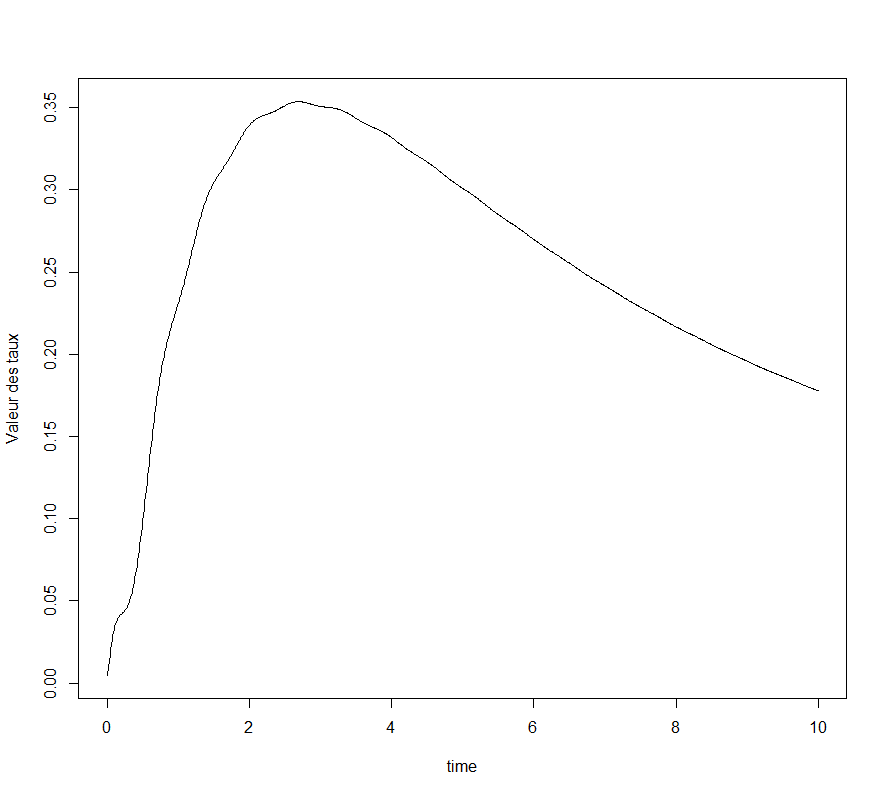
\includegraphics[scale=0.55]{courbe_des_taux_en_0}
        \caption{Simulation de la surface des taux en $t=0$ sur 10 ans}
\end{figure}

\noindent Nous obtenons bien une courbe des taux concave. Néanmoins, il se trouve que notre courbe de taux finit par être décroissante à partir de $3$ ans. Cette caractérisation contre intuitive est très probablement due à la paramétrisation de notre modèle.\\
\noindent Enfin, le graphique suivant représente la surface des taux.

\begin{center}
\begin{figure}[H]
         \centering 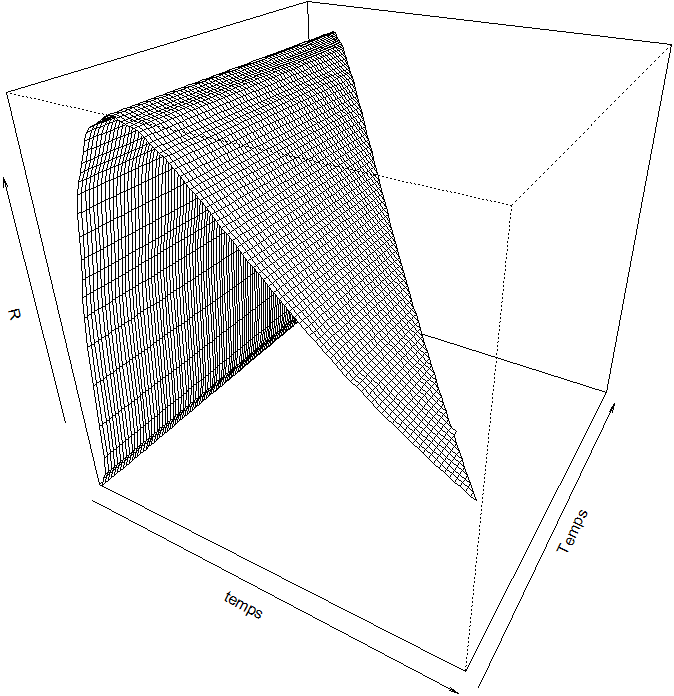
\includegraphics[scale=0.60]{R_surface}
        \caption{Simulation de la surface des taux R(temps,Temps) sur 10 ans}
\end{figure}
\end{center}

\section{Conclusion}

Naturellement, nous n'avons pas pu aller plus loin dans l'analyse financière de nos résultats car nous sommes limités par la sélection des paramètres. Pour calibrer un tel modèle,  on pourra citer "Calibration Methods of Hull-White Model" article de Sebastien Gurrieri, Masaki Nakabayashi et Tony Wong parut en 2011.

\nocite{*}
\bibliographystyle{plain}
\bibliography{biblio}

\pagebreak
\appendix
%\title{Annexes}
\section*{Annexes}
Ci-dessous le code que nous avons utiliser pour générer les graphiques. 
Nous avons utiliser une méthode de Monte-Carlo pour calculer les intégrales stochastiques du taux court, et les formules fermées démontrées ci-dessus pour calculer les zéro-coupons et la courbe des taux. 
\begin{center}
\begin{lstlisting}
## Simulation du brownien standard
T <- 1
n <- 100000
d <- T/n
w <- numeric(n)
for(i in 1:n) w[i+1] <- w[i] + d * rnorm(1)
## Graphique corespondant : 
plot.ts(w)
abline(h = 0)
#Donc W est un brownien sur [0;n]


# parametres du modele : 
.alpha = 0.5
.sigma = 1
.r0 = 0
vega <- function(t)
{
  return(1- sin(10*t)/(t+1))
}


#Fonction calculans le taux court r_t : 
r_t <- function(t,r0 = .r0,alpha = .alpha ,volatilite =1,periode_final=10,wienner=w)
{
  # condition d'arret
  if(t==0){
    return(r0)
  }
  
  # Integration prerequise
  max_iter <- length(w)
  somme_seq <- seq(0, round(max_iter*t/periode_final,0))
  N <- length(somme_seq)
  somme = 0
  for(i in 1:N)
  {
    somme = somme + exp(alpha * i * t / N) * w[i]
  }
  somme <- somme / N
  integrale_pour_wienner <- exp(alpha*t) * w[round(max_iter*t/periode_final,0)] - alpha * somme
  
  # return the result : 
  membre_2 <- integrate(function(u) return(exp(-alpha*(t-u))*vega(u)), lower = 0, upper = t)$value
  membre_3 <- volatilite * exp(-alpha*t) * integrale_pour_wienner
  return(r0*exp(-alpha*(t))+membre_2+membre_3)
}

#On implemente notre H&W
temps <- seq(0,10, length = 1000)
r_seq <- temps
for(i in 1:(length(temps)))
{
  r_seq[i] <- r_t(temps[i])
  print(c(1,i))
}
plot(temps[1:length(temps)], r_seq, type = "l", ylab = "r_t", xlab = "time")








#Fabriquons une courbe de taux
#On commence par creer la fonction qui nous donne les B(0,theta)
#B(0,theta) indexe par alpha

B <- function(t, T, alpha=.alpha, volatilite=.sigma)
{
  #condition d'arret
  if(T==0){return(1)}
  
  #prerequis
  A <- function(t,T,alpha=0.5){
    return((1-exp(-alpha*(T-t)))/alpha)
  }
  
  #lets go
  membre_1 <- r_t(t,0, alpha, volatilite)*A(t,T,alpha)
  membre_2 <- integrate(function(s) return(vega(s)*A(s,T,alpha)), lower = 0,  upper = T)$value
  membre_3 <- 1/2 * volatilite^2 * integrate(function(s) return(A(s,T,alpha)^2), lower = 0,  upper = T)$value
  return(exp(- membre_1 - membre_2 + membre_3))
}

# Maintenant faisont une courbe des taux zero coupon en t=0 d'echeance entre 0 et 10 : 
temps <- seq(0,10, length = 100) #t pouvant aller jusqu'a 10 ans ici
B_seq <- temps
for(i in 1:(length(temps)))
{
  B_seq[i] <- B(0,temps[i])
  print(c(2,i))
}
plot(temps[1:length(temps)], B_seq, type = "l", xlab = "time",  ylab = "B(0,T)")




# Passons a la courbe des taux : 

R <- function(t,T, alpha=.alpha,volatilite=.sigma)
{
  return((-1/T) * log(B(t,T,alpha,volatilite)))
}

# Et la courbe des taux en 0 est : 
temps <- seq(0,10, length = 100)
R_seq <- temps
for(i in 1:(length(temps)))
{
  R_seq[i] <- R(0,temps[i])
  print(c(3,i))
}
plot(temps[1:length(temps)], R_seq, type = "l", xlab = "time", ylab = "Valeur des taux")




## Maintenant, occupons nous de charter les ZC et la courbe des taux sur les deux parametres temps : 
temps <- seq(0,10, length = 100)
Temps <- seq(0,10,length=100)
mat <- matrix(NA,nrow=length(temps),ncol=length(Temps))
for (i in 1:length(temps)){
  for (j in 1:length(Temps)){
    if((temps[i]+Temps[j]) < 10){
      mat[i,j] <- B(temps[i],Temps[i])
      print(c(i,j))
    }
  }
}
persp(temps,Temps,mat,theta=30,phi=30)


## Ensuite, la surface des taux moyens continus : 
temps <- seq(0,10, length = 100)
Temps <- seq(0,10,length=100)
mat2 <- matrix(NA,nrow=length(temps),ncol=length(Temps))
for (i in 1:length(temps)){
  for (j in 1:length(Temps)){
    if((temps[i]+Temps[j]) < 10){
      mat2[i,j] <- R(temps[i],Temps[i])
      print(c(i,j))
    }
  }
}
persp(temps,Temps,mat,theta=30,phi=30)
\end{lstlisting}
\end{center}

\end{document}














